\glsresetall
 \graphicspath{{figures/analysing/}}
\chapter{Introduction}

The directivity of a sound sources is an issue that has an impact on many situations of our daily life, e.g. at live music venues. Voluntary listeners, namely the audience, enjoy comparatively high sound pressure levels when gathering around the stage. Non-voluntary listeners, generally neighbours, tend to perceive the sound emitted by the stage as a disturbing noise. This problem might be minimized with directivity control of the sound sources. The high sound energy will then be emits towards the audience, and less towards the neighbours. 


There are several effects that make this difficult, because commonly used loudspeaker contraptions for low frequency playback tend to act like omnidirectional sound sources. First, the dampening of sound in the air has significantly less influence on sound towards the lower frequency of the human hearing range than it has towards the higher frequency. Secondly, because of the way most houses are built, low frequency sound penetrates through walls and windows much more than high frequency sound. All of these effects lead to neighbours being disturbed by \textit{the low frequency} from nearby live music venues.\\
The difference in the perception of the sound is visualised in \autoref{fig:Problem}.


\begin{figure}[htbp]
	\centering
	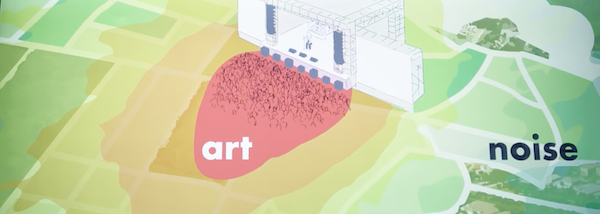
\includegraphics[width=1\textwidth]{change_later.png}
	\caption{Normalized \gls{spl} in colour, red is high \gls{spl} where blue is low \gls{spl}}
		\label{fig:Problem}
\end{figure}

%\autoref{fig:Problem} shows the total sound pressure level \gls{spl} in \gls{db} from \SI{20}{\hertz} to \SI{20}{\kilo\hertz} for the voluntary listeners and the non-voluntary listeners during a concert.
\autoref{fig:Problem} shows a qualitative drawing of a near-ideal sound pressure distribution in the vicinity of a stage during a concert. The high-\gls{spl}areas are highlighted by red color, and is the area where the voluntary listeners condense. This area is define as the \textbf{participants' area} The non-voluntary listeners are located in the area around the participants' area, that we define as \textbf{the neighbourhood}. 

While a \gls{spl} distribution as depicted in \autoref{fig:Problem} is easier to achieve the higher the frequency gets, towards low frequencies the \gls{spl}distribution might look more like depicted in autoref(fig:problem2).



The directivity control of mid- and high frequency has a known solution which has been applied for many years. In general, horns are used, which are designed for a particular radiation pattern. Due to the long wave length in the low/mid- and low frequency range, the horns that are required to direct those wavelengths are not feasible for practical applications due to their size and weight. Therefore other, more space saving solutions have been developed and implemented in the last decade. It is possible to achieve a cardiod emission pattern by arranging subwoofers in a particular manner. Two or three subwoofers are pointed towards the participants' area and one subwoofer is pointed the opposite way. The signal for the subwoofer pointing away from the audience is processed to manipulate the phase.


This project aims towards applying a principle that has been put into commercial use in the D\&B audiotechnik SL-series, where the low/mid frequency directivity is controlled by signal processing four speaker unit. Two units are arranged in the front of the line array module and the other two arranged on each of the sides of the line array module.



\section{preliminary problem statement}
The following questions are made with the intention of gathering the necessary knowledge, to be able to answer a later stated problem statement. The preliminary questions, which will be answered in the analysis, are:

\begin{itemize}
\item In which frequency area do the line source speaker behave omnidirectional?
\item Which known technique is used to do the speaker cardioid?
\item Can a simulation be made which support D\&B audiotechnik claim?
\end{itemize}




%%%
\part{Problem Analysis}\label{pt:analysis} \glsresetall
 \graphicspath{{figures/analysing/}}
	\chapter{Directional characteristics of a loudspeaker}\label{ch:directional}
		\section{Origin}\label{ch:polar_response}
Because this project is about shaping the directional characteristics of loudspeakers arrangements towards a particular direction, it is important to thorougly investigate the directional characteristic of a single loudspeaker. This serves as a baseline for comparison and also is essential, because the investigated loudspeaker will be used to form the speaker array later on.\\
In general, loudspeakers tend to display different directional behaviour depending on the frequency emitted. At low frequencies they can be viewed as omnidirectional sound sources. At higher frequencies the main direction of sound emission is in line with the motion direction of the voice coil. \citep[p. 910 f.]{crocker98}
Depending on the ratio of the emitted wavelength to the diameter of the speaker, a radiation pattern with side lobes can occur. An analytic approximation to the behaviour can be made  when looking at a vibrating piston in an infinite baffel. However, this only takes into account the front side of the speaker. It is difficult to incorporate the effects of an enclosure into this model.\\
There are possibilities to numerically model the sound field around a speaker in a cabinet. However in the context of this project, conducting a measurement seems to be the most favourable approach towards quantifying the sound pressure emitted by loudspeaker mounted in an enclosure. Measurements must be taken at numerous frequencies and positions along a circular trajectory.
For this project, measurements are conducted by placing the test object on a turntable in free field conditions and measuring transfer functions with a microphone. The voltage output of the amplifier and the gain of the microphone can be calibrated so that the only part unknown is transduction performed by the test object. The results of this sort of measurement contain several transfer functions in frequency domain and corresponding impulse responses in time domain. Because they will often be visualized in polar plots, they will henceforth be refered to as the \textit{polar response}.
The knowledge gained through measuring the polar response can then be used in order to designate a feasible frequency range for beamforming in the way that will be described later on. 

\section{Transfer Function Measurement with Sweeps}\label{sec:sweep_theorie}
The characterization of the directional behaviour of the speaker consists of a large number of transfer function measurements. While there are many methods available to obtain transfer functions, it was decided to go with a method that is based on sweeps, due to several benefits. \citep[p. 3 ff.]{mueller01}\\
The sweep signal used for the measurement can be generated by the \gls{ift} of a desired spectrum and a group delay that is designed accordingly. This results in a sinusidal waveform with a continuously altering frequency. In most cases it is desirable to keep a nearly constant amplitude over the whole length of the sweep. The procedure of generating such a sweep signal is illustrated in \autoref{fig:sweep_signal}.

\begin{figure}[htbp]
	\centering
	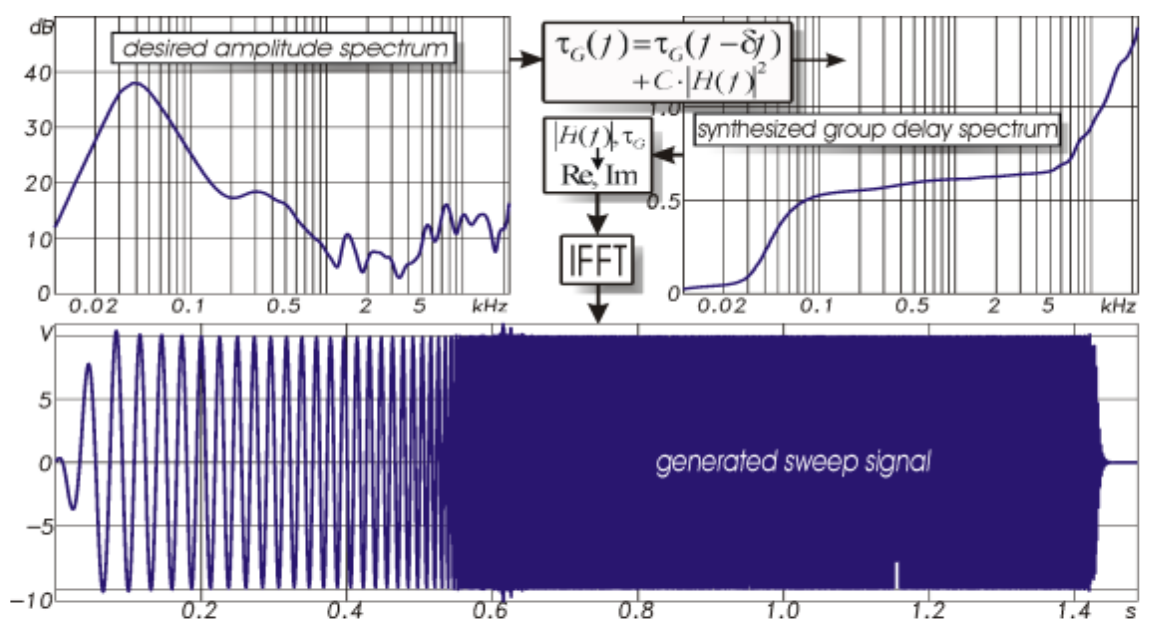
\includegraphics[width=1\textwidth]{mueller01_sweep.png}
	\caption{Sweep synthesis with arbitrary spectral magnitude and nearly constant envelope, taken from \citep{mueller01}}
		\label{fig:sweep_signal}
\end{figure}

The test signal is played back via the loudspeaker that is the test object and the sound is recorded with a microphone in a particular angle towards the main axis of the loudspeaker. An \gls{fft} is performed on the recorded signal. The transfer function of the loudspeaker is then calculated by a multiplication operation with the recorded signal and the inverse of the test signal in frequency domain. It has to be taken into account, that not only the properties of the loudspeaker, but also the distance between the loudspeaker and the microphone and the sound field in the room have an influence on the measurement results. In the context of this project is therefore expedient to conduct the measurements in free field conditions, which means resorting to an anechoic chamber.\\
One particular advantage of sweep measurements over other methods to determine the transfer function is that nonlinearities in the measurement chain or the \gls{dut}, that lead to distortion, can be isolated from the measured transfer function and can be assessed seperately. \citep[p. 20 f.]{mueller01} Simply put, this property is due to the fact, that in the sweep signal, every frequency has a certain group delay, which leads to harmonics being displayed at a negative time when the test signal and the measured signal are convolved in time domain. While it is not the subject of this project to investigate nonlinearities in the behaviour of the speaker in depth, keeping track of the distortion helps with keeping the gains in the measurement chain at a good operating level.

\section{Measurement Setup}\label{sec:meas_setup}
In order to obtain the polar response, transfer functions have to be measured at numerous points. To make measurements more time efficient the loudspeaker is placed on a turntable. The acoustical center (see also \autoref{sec:ac_center}) the loudspeaker is placed on the turning axis. The gain on the microphone amplifier and the input of the soundcard are calibrated, so that a known digital value at the soundcard corresponds to a known sound pressure at the microphone membrane. The gain of the power amplifier that drives the speaker is adjusted, so that a known value at the output of the soundcard corresponds to a known voltage over the terminals of the speaker. With these prerequesits the transfer function can be quantified as sound pressure per voltage at a given distance. The rotation of the turntable, on which the loudspeaker is placed, is controlled by the measurement routine on the computer. After every transfer function measurement, the orientation of the loudspeaker is altered, so that the measurement angles are evenly distributed along the circumference. The measurement data are stored, so that they can be processed into a readable form subsequently.


\begin{figure}[H]
	\centering
\begin{picture}(0,0)%
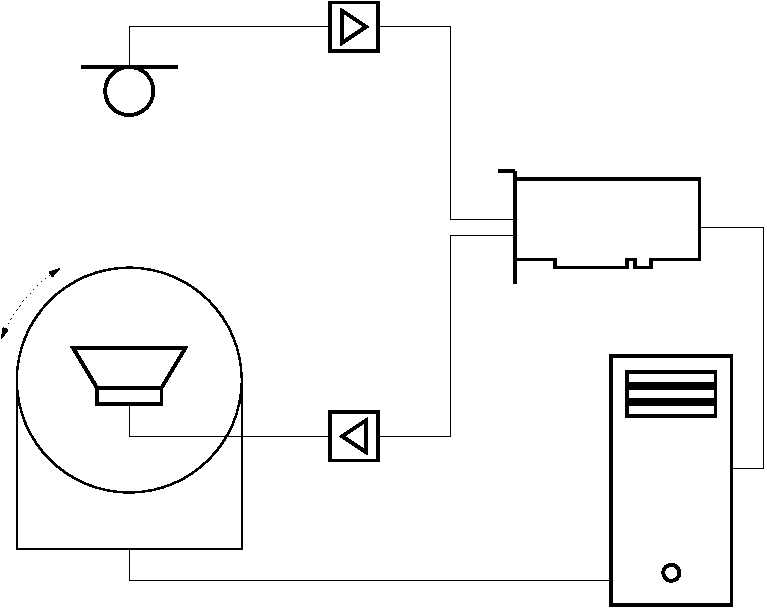
\includegraphics{meas_setup_01.pdf}%
\end{picture}%
\setlength{\unitlength}{2818sp}%
\begingroup\makeatletter\ifx\SetFigFont\undefined%
\gdef\SetFigFont#1#2#3#4#5{%
  \reset@font\fontsize{#1}{#2pt}%
  \fontfamily{#3}\fontseries{#4}\fontshape{#5}%
  \selectfont}%
\fi\endgroup%
\begin{picture}(8570,6816)(3053,-7474)
\put(4900,-1771){Microphone}%
\put(6525,-1501){Amplifier}%
\put(3250,-7081){Turntable}%
\put(6525,-6091){Amplifier}%
\put(9125,-3211){Sound Card}%
\put(10025,-6361){Computer}%
\end{picture}%
\caption{Measurement setup for transfer functions; for convenience the loudspeaker is placed on a turntable, that is controlled by the measurement routine on the computer.}
\label{fig:measurement_setup}
\end{figure}

\section{Determining the Acoustic Center of the \gls{dut}}\label{sec:ac_center}
In order to achieve meaningful results regarding the directional characteristic of the a loudspeaker, it is necessary to know the location of the  acoustic center of the loudspeaker.
In \citep{ansis1.1}, the ``effective acoustical center'' of an electroacoustical transducer is defined as the ``position of the effective or virtual point source from which sound pressure varies inversely as distance''. This concept is further discussed in \citep{jacobsenetal}, where the authors also state, that the position of the acoustic center is frequency dependent. For gathering the data to characterize the directivity it is desirable to position the acoustic center of the \gls{dut} on the rotational axis if the turntable. This can lead to practical difficulties due to the frequency dependency. It is therefore necessary to assess the position of the acoustical center of the \gls{dut} in the desired frequency range via a measurement.\\

Appendix \ref{ax:directional_1} shows the results of a measurement of the polar response that has been conducted without knowing the position of the acoustic center of the \gls{dut} that has been used.
When analyzing the phase data plotted in \autoref{fig:02_23_phase} it seems rather obvious, that the acoustic center of the \gls{dut} has been in front of the rotational axis of the turntable. 
It appears to be possible to estimate the position of the acoustic center by exploiting, that both wavelength and phase at the measurement points on the main axis (\SI{0}{\degree}) and in the opposite direction are known. As described beforehand, the concept of an acoustical center is tied to a  point source, from which waves appear to emerge. If the acoustical center is placed  on the rotational axis, the phase at all microphone positions should have the same value. In the given case it is assumed, that the acoustical center is only off the rotational axis in only the direction of the main axis of the \gls{dut}, and not shifted to the side.
The difference of the phase angles at \SI{0}{\degree} and \SI{180}{\degree} at a given frequency therefore corresponds to a proportion of the wavelength that is double of the distance that the \gls{dut} has to be shifted backwards in order to move the acoustical center onto the rotational axis.
\begin{equation}
S\,=\,\frac{1}{2}\cdot\frac{\phi_0-\phi_{180}}{360^\circ}\cdot\lambda
\end{equation}
\startexplain
    \explain{$S$ is the distance that the \gls{dut} has to be shifted backwards}{\si{m}}
    \explain{$\phi_0$ is the phase angle at the main axis}{\si{\degree}}
    \explain{$\phi_{180}$ is the phase angle at \SI{180}{\degree}}{\si{\degree}}
    \explain{$\lambda$ wavelength}{\si{m}}
\stopexplain    
If \(S\) takes on a negative value, the acoustical center is behind the rotational axis and the \gls{dut} has to be shifted towards the front. There are constraints to the applicability of this concept. The frequency, on which the calculation is based, has to be inside the frequency range at which the speaker can be considered omnidirectional.
The wavelength of the measured frequency can be problematic when it is very long, as the phase difference \(\delta\phi\) between \(phi_0\) and \(phi_{180}\) becomes comparatively small. This leads to a bigger influence to the uncertainty of the phase measurement. On the other hand, comparatively short wavelengths may lead to aliasing effects, when there is a big offset of the center from the rotational axis. However this does not to be so relevant in practical application, because towards higher frequencies, loudspeakers tend not to behave like omnidirectional sources.\\
In \autoref{tab:shift_meas1}, data from the measurement described in Appendix \ref{ax:directional_1} has been used to calculate the offset of the acoustical center from the rotational axis of the turntable at three different frequencies. The wavelengths \(\lambda\) were based on the assumption, that the speed of sound was \(c\,=\,\)\SI{343}{\meter\per\second}, corresponding to a temperature \(T\,\approx\,\)\SI{20}{\celsius}. The results for all three frequencies are rather similar.
\begin{table}[H]
\centering
\caption{Calculation of the offset of the acoustic center based on Appendix \ref{ax:directional_1}}
\label{tab:shift_meas1}
\begin{tabular}{|lr|r|r|r|}
\hline
Frequency              & {[}Hz{]}  & 60    & 100    & 150    \\ \hline
\(\phi_0\)             & {[}Deg{]} & 58.8  & 341.1  & 266.1  \\ \hline
\(\phi_{180}\)         & {[}Deg{]} & 17.2  & 269.7  & 159.9  \\ \hline
\(\Delta\phi\)         & {[}Deg{]} & 41.6  & 71.4   & 106.2  \\ \hline
\(\lambda\)            & {[}m{]}   & 5.72  & 3.43   & 2.29   \\ \hline
\(S\)                  & {[}m{]}   & 0.330 & 0.340  & 0.337  \\ \hline
\end{tabular}
\end{table}
Comparing \(S\) with the positioning of the speaker relative to the rotational axis during the measurement would allow for specifying the estimated position of the acoustic center. However, there was some significant undesired mechanical flexibility in the way the speaker was mounted, which lead to imprecisions (see \autoref{fig:setup_02_23}). Therefore, another mechanical solution was implemented and the measurement was repeated. This is  logged in Appendix \ref{ax:directional_2}.
During this second measurement campaign the speaker was placed further to the back to get the acoustical center closer to the rotational axis. However, there is still some offset, as can be seen in \autoref{tab:shift_meas2}.
Adding \(S\) to the distance between  the front plane of the cabinet and the rotational axis, a rough estimate of the position of the acoustic center in relation to the front plane of the cabinet \(C\,\approx\,\)\SI{0.17}{\meter} can be made. As there were still some mechanical weaknesses involved and the temperature during the measurement was unknown, this estimate has to be confirmed in a final measurement campaign, where the speaker is set back according to the findings of \autoref{tab:shift_meas2}.\\
One aspect that has to be mentioned in this context is the dependency of the acoustic center on frequency. According to the findigs of \citep{vanderkooy10}, who has done a boundary-element calculation of the acoustic center, the frequency dependent position alteration can be deemed  neglegible for the sake of this project.
\begin{table}[H]
\centering
\caption{Calculation of the offset of the acoustic center based on Appendix \ref{ax:directional_2}}
\label{tab:shift_meas2}
\begin{tabular}{|lr|r|r|r|}
\hline
Frequency              & {[}Hz{]}  & 60    & 100    & 150   \\ \hline
\(\phi_0\)             & {[}Deg{]} & 108.9 & - 60.8 & 138.0 \\ \hline
\(\phi_{180}\)         & {[}Deg{]} & 103.3 & - 70.8 & 126.5 \\ \hline
\(\Delta\phi\)         & {[}Deg{]} & 5.6   & 10     & 11.5  \\ \hline
\(\lambda\)            & {[}m{]}   & 5.72  & 3.43   & 2.29  \\ \hline
\(S\)                  & {[}m{]}   & 0.044 & 0.048  & 0.037 \\ \hline
\end{tabular}
\end{table}
%A way to determine the acoustical center by measurement can be proposed as follows. The loudspeaker is placed on the turntable, oriented with its main axis directly towards the measurement microphone (\SI{0}{\degree}). Details about this procedure can be found in \autoref{ax:directional_1}.


\section{Determining the beamwidth of the \gls{dut}}\label{sec:ac_center}
In order to find the beamwidth of the \gls{dut}, a pre polar response measurement have to be done to localize the acoustic center of the \gls{dut} by analyse the polar phase of the \gls{dut}. With the knowledge of the polar phase to a given frequency, it is possible to calculate the distance in x and y direction, the \gls{dut} have to be moved. The pre polar response is explained in \autoref{ax:directional_1}, and in \autoref{} the moment was calculated to ... in x direction and ... in y direction. 
After the speaker is moved to the calculated position, the polar response is measured again and analysed in \autoref{ax:directional_2}. Because of flexibility of the first stand in \autoref{ax:directional_1}, the position of the speaker is of with \SI{4.5}{\centi\meter} to the front. The measurement  is executed according to \autoref{appendix:beamwidth} and the beamwidth of the \gls{dut} is as following \autoref{fig:beamwidth_offset_4.5_cm} 

\begin{figure}[htbp]
	\centering
	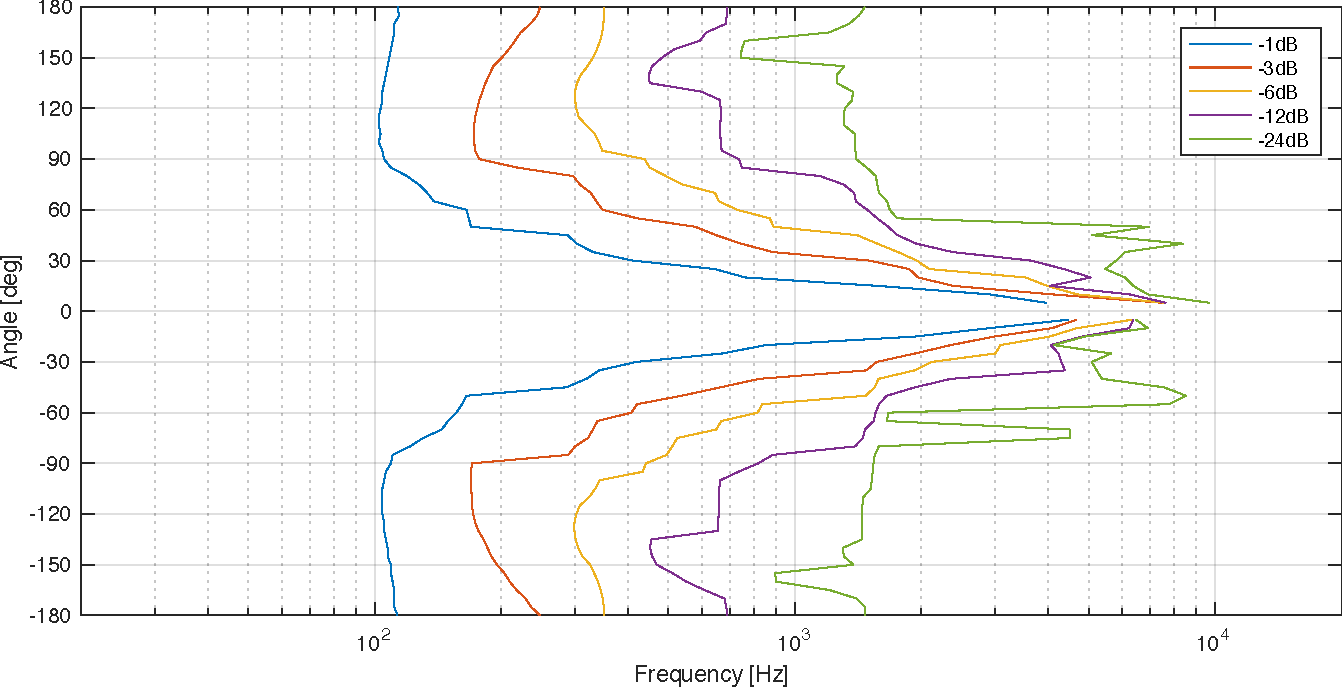
\includegraphics[width=1\textwidth]{beamwidth_off_4_5_cm.pdf}
	\caption{The figure shows the beamwidth to a specified \si{\decibel} change between the front measurement and a measurement from a given angle of the \gls{dut}. It find the first frequency where the \gls{spl} difference between front measurement and the measurement from the given angle is $n$\si{\decibel}, where $n$ is given in the figure. The \gls{dut} which correspond to this figure is a \citep{seas33}}
		\label{fig:beamwidth_offset_4.5_cm}
\end{figure}

	\chapter{Analytical descriptions}\label{ch:analytical}
		\section{Single source}\label{ch:single_speaker_source}
To gain understanding about the interaction of several sources emitting sound simultaneously it is essential to first investigate the behaviour of a singular sound source. In the context of this project loudspeakers are investigated. The goal of this section is to find a way to represent the sound emission of loudspeakers within the frequencies boundaries of this project (\SIrange{60}{300}{\hertz}).
The representation must be suffiencently accurate yet relatively simple to calculate in order to be useful in the optimization process that is a later part of this project (see \autoref{ch:optimization}).

%This section aims to introduce and analyse the fundamental for a single source, by analyse the behaviour of a baffled circular plane piston source. The pressure around the piston source will be analysed analytically, to determine the radiation of a single speaker from \SI{60}{\hertz} and upwards and compare it with the measurement from \autoref{ch:polar_response}. The \SI{60}{\hertz} lower limit enable the simulation to be validated by measurement in the AAU anechoic chamber and is a used lower limit for the low/mid driver in some line source array \citep{V-DOSC}.  The analyse shall end out with a approximated simulation model of the \gls{dut}.
\subsection{Pressure emission from an omidirectional source}
As explained in \autoref{ch:polar_response} loudspeakers are commonly treated as omnidirectional sources at low frequencies. Taking advantage of this approximation, the sound pressure emission in free field conditions can be described conveniently. \citep[p. 171]{Kinsler2000} state the following equation \autoref{eq:omni_source} for a pulsating sphere. It has to be noted, that the position of the sphere in the given case is the acoustic center of the loudspeaker (see \autoref{sec:ac_center}).
\begin{equation}\label{eq:omni_source}
p(r,t)\,=\,\rho_0 c V_0 \left(\frac{a}{r}\right)\cos \theta_a \textbf{\textit{e}}^{j\left(\omega t - k(r-a)+\theta_a\right)}
\end{equation}
\startexplain
\explain{$p$ is the sound pressure.}{\si{\pascal}}
\explain{$r$ is the distance, for which the pressure is being calculated, \(r>a\).}{\si{\meter}}
\explain{$t$ is the time, for which the pressure is being calculated.}{\si{\meter}}
\explain{$\rho_0$ is the specific density of air.}{\si{\kilo\gram\per\cubic\meter}}
\explain{$c$ is the speed of sound.}{\si{\meter\per\second}}
\explain{$V_0$ ist the peak velocity at the surface of the spherical source.}{\si{\meter\per\second}}
\explain{$a$ is the radius of the spherical source.}{\si{\meter}}
\explain{$\theta_a$ is equal to $\tan(ka)$.}{\si{1}}
\explain{$\omega$ is the angular frequency.}{\si{\second^{-1}}}
\explain{$k$ is the wavenumber.}{\si{\meter^{-1}}}
\stopexplain

\subsection{Pressure emission from a baffled piston}
Another  approach to analytically approximate the behaviour of a cone loudspeaker is given by \citep[p. 179 ff.]{Kinsler2000}, where the behaviour of the sound radiated from a plane circular piston surrounded by an infinte rigid baffle is described.


%To characterize the directional properties of an analytical model of the \gls{dut}, the source will be modulated in two dimension as one baffled circular plane piston source. The analysis of a piston source in two dimension built on a thin piston source in three dimension where the x axis is fixed in the plot. This is possible because of vertical beam patten symmetry of \autoref{fig:continues_line_source} \citep{Kinsler2000}. The piston lays flat down so i look like a line source and have radius $a$. The baffled circular plane piston source can be considered as many continuous line sources, which detonate dx and is pointing towards the reader on \autoref{fig:continues_line_source}. The calculated pressure point will be in far field where $r>>a$ holds and the surface integral can be rewritten to a Bessel function \citep{Kinsler2000}. The pressure formula is therefore:

\begin{equation}
p(r,\theta ,t)=\frac{j}{2} \rho_{0}c  V_{0}\frac{a}{r}ka \left ( \frac{2J_1(ka\, sin(\theta ))}{ka\, sin(\theta )} \right )e^{j(\omega t-kr)}
\end{equation}
Where the complete surface vibration is described with

\begin{equation}
v = V_{0} \cdot exp(j \omega t)
\end{equation}

\startexplain
    	\explain{$v$ is the complex speed of the line source }{\si{1}}
        \explain{$V_{0}$ is the Amplitude}{\si{1}}
        \explain{$j$ is the imaginary unit }{\si{1}}
        \explain{$\omega$ is the angular velocity }{\si{1}}
        \explain{$t$ is the time }{\si{1}}
\stopexplain
    
Each small sources is treated as an baffled simple source with a width of $dx$ and the source strange can be modulated as following      

\begin{equation}
dQ = V_{0} 2 a\, sin(\phi) \, dx
\end{equation}

    \startexplain
    		\explain{$dQ$ is the simple source strange }{\si{1}}
        \explain{$V_{0}$ is the Amplitude}{\si{1}}
        \explain{$a$ is the radius for cylinder }{\si{1}}
        \explain{$\phi$ is the angle between the radius $a$ and the x axis}{\si{1}}
        \explain{$dx$ is the length for the simple source }{\si{1}}
    \stopexplain    
 
The following \autoref{fig:continues_line_source} shows an example of the continues line source where one of the small source is showed with width $dx$ and length $2a \, sin(\phi)$. 

\begin{figure}[H]
	\centering
\begin{picture}(0,0)%
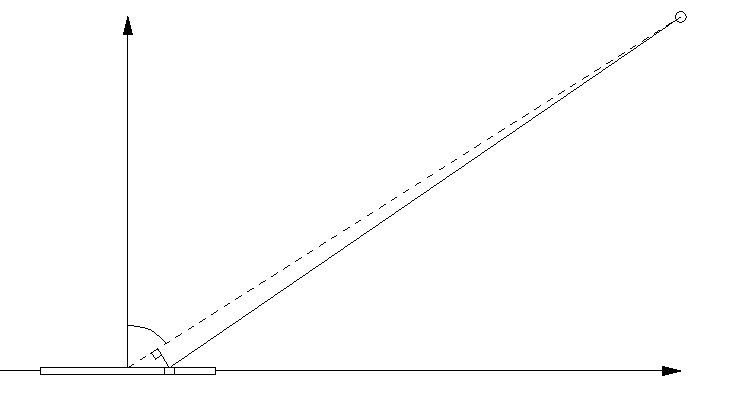
\includegraphics{line_source.pdf}%
\end{picture}%
\setlength{\unitlength}{746sp}%
%
\begingroup\makeatletter\ifx\SetFigFont\undefined%
\gdef\SetFigFont#1#2#3#4#5{%
  \reset@font\fontsize{#1}{#2pt}%
  \fontfamily{#3}\fontseries{#4}\fontshape{#5}%
  \selectfont}%
\fi\endgroup%
\begin{picture}(31223,16833)(-5411,-436)
\put(12106,7139){r'}%
\put(24121,15599){P(r,$\theta$,t)}%
\put(946,2684){$\theta$}%
\put(23851,659){x}%
\put(-89,16094){z}%
\put(11341,8354){r}%
\put(3466,-571){$a$}%
\put(1441,-376){$dx$}%
\put(-134,-421){0}%
\put(-4049,-571){$-a$}%
\put(226,1649){$\Delta$r}%
\end{picture}%
	\caption{The model of a continues line source where y axis is pointing towords the reader. (ref the book)}
		\label{fig:continues_line_source}
\end{figure}




\subsection{Simulation of the \gls{dut} as a piston source and compare to measurement in \autoref{ch:polar_response}}
In this section, the \gls{dut} will be simulated as a baffled circular plane piston source as described in \autoref{ch:single_speaker_source} and compared to the actually measurement of the \gls{dut} \autoref{ax:directional_2}. An piston simulated model of \citep{seas33} in MATLAB shows in \autoref{fig:piston_model_of_seas33}

\begin{figure}[H]
	\centering
	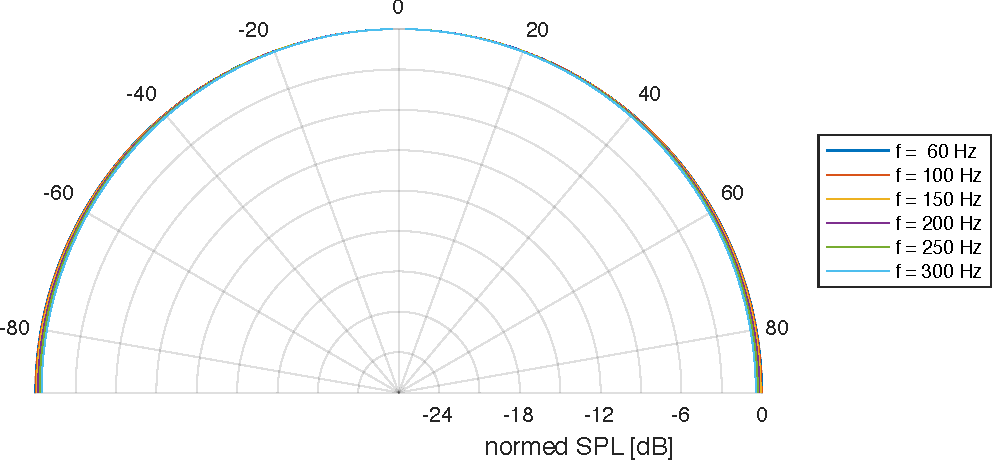
\includegraphics[width=0.8\textwidth]{piston_model.pdf}
	\caption{The figure shows  The \gls{dut} which correspond to this figure is a \citep{seas33}}
		\label{fig:piston_model_of_seas33}
\end{figure}

The actually measurement of the \citep{seas33}  \autoref{ax:directional_2}.

\begin{figure}[H]
	\centering
	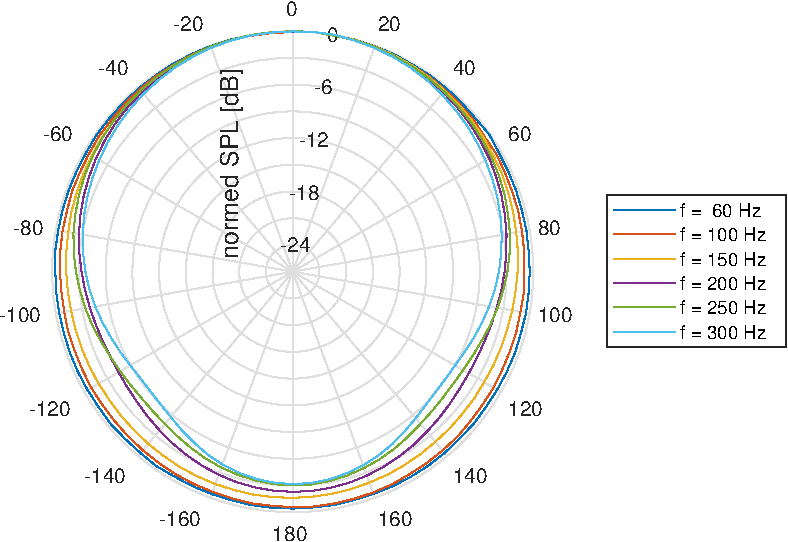
\includegraphics[width=0.8\textwidth]{meas1_seas.pdf}
	\caption{The figure shows  The \gls{dut} which correspond to this figure is a \citep{seas33}}
		\label{fig:speaker_model}
\end{figure}

\subsection{Conclusion}
		\section{The 300 \gls{hz}}
		\section{The dimension limit} 
	\chapter{Numerical Simulation}\label{ch:numerical}   



%%
\part{Design and Optimization}\label{pt:design} 
\graphicspath{{figures/design/}}
	\chapter{Hardware Configuration}
		%\section{Digital Signal Processor Choice}

The chosen component is the \gls{dsp} for numerous reasons that are going to be presented in the following subsections.

\subsection{Advantage of the \gls{dsp} over the FPGA}

Some of the  reasons of choosing a \gls{dsp} over an FPGA in this project are:
 
\begin{itemize}

\item  The simplicity of designing with a \gls{dsp} due to the availability of all the simple functionalities in a micro-controller \citep{eetimes}. 

\item A \gls{dsp} is designed to perform signal processing tasks unlike the FPGA which purpose of creation was not related to signal processing but to program circuits \citep{eetimes}. 

\item A \gls{dsp} is more suitable in terms of cost/performance, when the application has less than 3000 \gls{mmac} per second, which means that it is better for low demanding applications \citep{eetimes}. 

\item FPGA's lack integrated DAC and ADC \citep{eetimes}. 

\item The \gls{dsp}'s are more power efficient than the FPGA's which can be important if the effect is to be used on the move on battery power \citep{rtcmag}. 

\item A \gls{dsp} can be optimal if there are many operations that are repeated \citep{eetimes} \citep{hunteng}. 

\end{itemize}

\subsection{Advantage of the \gls{dsp} over the Raspberry Pi}

Some of the  reasons of choosing a \gls{dsp} over a Raspberry Pi in this project are:
 
\begin{itemize}

\item \gls{dsp}'s are much faster for integer and floating mathematical calculations. \gls{dsp}'s are designed to compute large and complex operations that are repetitive which makes it more suitable for this project \citep{diffbet} \citep{esp_simone}.   

\item A micro-controller, such as a Raspberry Pi, has many different features that are not going to be used in the project \citep{diffbet} \citep{esp_simone}. 

\item In general, a \gls{dsp} is faster than a micro-controller, for signal processing, because it involves specialized units like multipliers \citep{diffbet2}. 

\item A micro-controller is usually used for control applications and not signal processing even if it can work \citep{tex_dsp}.

\end{itemize}












	\chapter{Optimizing SP-Parameters}
	\chapter{Implementing SP-Parameters}


%%

\part{Test and Discussion}\label{pt:test}
\graphicspath{{figures/tests/}}
	\chapter{Performance Evaluation}
		%In this section, all tests will be made and the fulfillments will be marked in a table in the end of each test section, where the following marks will indicate if the test is approved, conditionally approved or not fulfilled.
 \vspace{1cm}
    \startexplain
     \explain{\cmark  \hspace{4mm} is approved}{$\cdot$}
     \explain{\cmark* \hspace{1mm} is conditionally approved}{$\cdot$}
     \explain{\xmark \hspace{5mm} is not fulfilled}{$\cdot$}
    \stopexplain
	\chapter{Comparison: Simulations and Measurement}
	\chapter{Comparison: Array vs Single Speaker}


 
%%
\part{Conclusion}\label{pt:conclusion}
%\section{Discussion}\label{sec:discussion}

In \autoref{pt:tests} all the requirements were tested to see if they can be approved. It is seen that out the 26 stated requirements, 16 are approved, six are partially approved and four are not approved.
\autoref{req:delay1} is approved, but some additions have to be made to make it function as a usable delay effect. The reason of this is that the time between the echoes is too short. With the implemented buffer size it is only possible to produce a delay time of \SI{41}{\micro\second}, which is too short. 
The six requirements that are partially approved are all related to the missing user interface. The user interface was not implemented due to the time limit of the project and the fact that it was chosen to make the implementation of the effects the main focus. The six partially approved requirements are categorized as such, because it is possible to change the required parameters, but only through changing them directly in the program. 
The first requirement that is not approved is \autoref{req:SNR}. It was measured that the \gls{dsp} has a \gls{snr} of \SI{39.91}{\decibel}, which is lower than the \gls{snr} in the guitar. The low \gls{snr} in the \gls{dsp} means that it will not even be enough to re-design the effects to make them as noiseless as possible.  
The second requirement that is not approved is \autoref{req:power2}, where the reason is that the \gls{dsp} is powered by a \SI{5}{\volt} USB supply. Since the supply voltage that is now used is smaller than the stated \SI{9}{\volt}, this requirement can be approved if a \SI{9}{\volt} supply is used to make a \SI{5}{\volt} supply for the \gls{dsp}.
The third and fourth requirement that are not approved are \autoref{req:flanger1} and \autoref{req:chorus1}. The reason of this is that the implemented \gls{cordic} algorithm is not able to produce sine waves with lower frequencies than \SI{0.4}{\hertz}, because with 32-bit precision sine and cosine values for frequencies less than \SI{0.4}{\hertz} can not be represented. A solution to this would therefore be to use a higher bit precision. \\
%The fifth requirement that is not approved is \autoref{req:preamp3}, because the measured output impedance of the preamp is measured to \SI{9.06}{\kilo\ohm}, which should be smaller than \SI{2}{\kilo\ohm}. The result of the measurement is questionable because the output impedance of an \gls{opamp} normally lies around \SI{50}{\ohm} to \SI{200}{\ohm}. \\

Some choices than were made in the development of the project can be discussed. One of them is the decision of implementing all the effects entirely in assembly. The reason behind the decision was to make the effects run as fast as possible, to get familiar with the assembly language, and to get a better understanding of the \gls{dsp}. It is seen in \autoref{app:effect_run_time}, that each effect uses approximately one tenth of the sampling period to complete its program. This indicates that it might have been possible to implement parts of effects in the slower, but faster implementable language C. This approach might have left time for implementing the user interface for instance. 
Another discussion is whether the resolution of the calculations in the effects should be increased from 16- to 32-bits. This will improve the sound quality of the effects. It was seen in the development of the \gls{cordic} calculations that increasing the precision, made it possible to to produce sine waves of lower frequencies. The resolution could of course always be a parameter that could be improved, but the noticeable difference from going from 16- to 32-bits, might be larger going from 32- to 64-bits. It has to be taken into account that higher resolution would require more memory.  
A subject for discussion is the approach for developing the effects, the \gls{reverb} for example. In this specific case, a Moorer \gls{reverb} unit was chosen. The reason of this decision was to have some guidelines for developing a \gls{reverb} effect. When looking back, it might have been beneficial to design the effect without relying as much on a reference. This might have improved the possibility  of making the effect sound as intended. \\

For further enhancements, several steps could be made towards improving the product. One of them is the user interface, which would not only make it possible to approve more of the requirements, but also make the final product more usable. One would for example not have stop and reprogram the \gls{dsp} to change effect, or even to just change one parameter in an effect. 
Additional developments can also be finishing the implementation of the designed effects but also the missing parts in the already implemented ones in assembly, such as implementing the attenuating part of the equalizer or making the \gls{cordic} algorithm able to produce different oscillations at the same time to finish the chorus effect. 
Moreover, a parameter that can be investigated more is the noise in the system. It could be investigated if it in some way is possible to improve the \gls{snr} in the \gls{dsp}. 
%

\glsresetall
\appendix % Start of appendix
\addtocontents{toc}{\protect\setcounter{tocdepth}{0}} 
%\input{chapters/appendices/_appendices} % Include appendices
%Appendix:

 \graphicspath{{figures/appendix/}}
\part{Appendix}\label{pt:appendix}
\section{Outline ...}
In this appendix the control of the Outline turntable will be descriped    
